\documentclass[man,floatsintext]{apa6}

\usepackage[american]{babel}

\usepackage{csquotes}
\usepackage[style=apa,sortcites=true,sorting=nyt]{biblatex}
\DeclareLanguageMapping{american}{american-apa}
\addbibresource{../LaTeX/Bibliography.bib}
\usepackage{hyperref}

\title{Comparing Charter \& Traditional Public Schools Using Propensity Score Analysis}
\shorttitle{Comparing Charter \& Traditional Public Schools}

\author{Jason M. Bryer}
\affiliation{University at Albany, SUNY}
\note{\href{http://jbryer.github.com}{jbryer.github.com}\\ \href{mailto:jason@bryer.org}{jason@bryer.org}}
\authornote{Paper presented at the 2012 AERA Annual Meeting on April, 15, 2012 in Vancouver, British Columbia, Canada. This paper represents the results of a pilot study done using the 2007 NAEP for a dissertation that will utilize the 2009 NAEP. Only a subset of the figures and tables are provided here. The full set of tables and figures can be obtained at \url{http://github.com/jbryer/Dissertation}.}

\leftheader{Bryer}

\abstract{The use of propensity score analysis \parencite{RosenbaumRubin1983} has gained increasing popularity for the estimation of causal effects within observational studies. However, its use in situations where data is multilevel, or clustered, is limited (Arpino \& Mealli, 2008; Hong \& Raudenbush, 2006; Thommes \& West, 2011). This study will introduce the \texttt{multilevelPSA} \parencite{multilevelPSA} package for R that provides functions for estimating propensity scores for large datasets using logistic regression and conditional inference trees. Furthermore, a set of graphical functions that extends the framework of visualizing propensity score analysis introduced by \textcite{psagraphics} to multilevel analysis will be discussed. An application for estimating the effects of charter schools as compared to traditional public schools on reading and mathematics in grades 4 and 8 is provided.}

\keywords{charter schools, propensity score analysis, multilevel analysis}

\begin{document}
\maketitle

The concept of school choice within the United States is not new. Private schools have been educating students since the founding of the United States. However, in 1988, Ray Budde proposed an alternate approach to school choice that has grown to be known as charter schools \parencite{Kolderie2005}. Unlike their private school counterparts, charter schools receive public funding, but they are relieved of many of the bureaucratic and regulatory constraints public schools adhere to, but are still held accountable for student performance. Despite claims by charter school advocates that charter schools are performing as well if not better than the public school counterparts \parencite[see e.g.][]{AllenConsolettieKerwin2009}, studies provide mixed results with regard to charter school performance \parencite[see e.g.][]{BraunJenkinsGrigg2006,credo,HubbardKulkarni2009}. Ultimately, there is agreement that more research is necessary to address the question of whether charter schools provide substantially better academic experiences for students. This study will investigate the question of whether students who attend charter schools outperform their public school counterparts on two key academic domains: reading and mathematics.

\begin{figure}[tp]
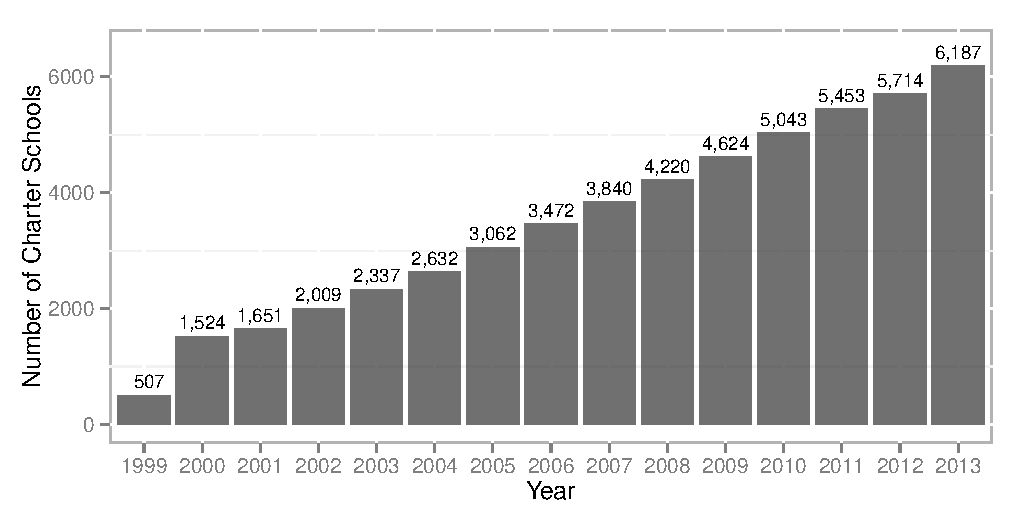
\includegraphics[width=\textwidth]{../Figures/CharterSchoolGrowth.pdf}
\caption{Charter School Growth 1999-2008}
\label{fig:charterSchoolGrowth}
\end{figure}

At the center of the charter school debate is an issue that has concerned thinkers for centuries, the question of how to support causal inferences. In this context we aim to assess the effect of a treatment on a measurable outcome using observational data. Traditionally, randomized experiments have been considered the ``gold standard'' for studying questions of causality. In the context of this study, and many other questions in education randomization is either impractical or unethical. This means that observational studies are often essential to support inferences about whether treatments influence outcomes.

However, lacking randomization, observational studies nearly always invite selection bias. Charter schools are, by definition, schools of choice. In observational data contexts, simple comparisons of two groups such as public and charter schools cannot help but ignore the inherent and systematic differences between the two groups. However, with an appropriately designed observational study, and an appropriate analysis, the effects of the selection bias can be taken into account in a way that simple comparisons are replaced by adjusted comparisons of groups. This is done utilizing a class of statistical procedures introduced by \textcite{RosenbaumRubin1983} called propensity score analysis.

Propensity score analysis has seen considerably increased use in the social sciences within the last few years \textcite{ThoemmesKim2011}. However, its use in situations where multilevel, or clustered data are of interest, have been limited \parencite{ArpinoMealli2008}. Using data from the 2007 National Assessment of Educational Progress (NAEP) for mathematics and reading at grades four and eight, estimates of the differences between charter and public schools will be calculated at two levels, namely state and national. Given the variability of charter schools laws across states, it is important to consider the impact of clustering. Analysis will be conducted using the multilevelPSA package in R \parencite{rdevelopment}. Specifically, propensity scores will be estimated within each state and these will be used for matching or stratification of students within each state. Comparisons of specific students, or groups of students, will in all cases be within states. Effects will then aggregated to provide state and national effect estimates.

\section{Method}
	
As with all propensity score analyses, it is preferable to utilize multiple methods for estimating propensity scores \parencite[see e.g.][]{Stuart2010}. Most of the studies conducted using PSA involve analysis in two phases where phase one involves the calculation of propensity scores or matching for both treatment and control units of analysis; and phase two involves the comparison of those two groups. However, there is little research with regard to situations where data is multilevel. As such, this study will be organized as such:

\begin{enumerate}
	\item \textit{Propensity score analysis using stratification.} This method ignores state assignment as a clustering variable. Under this broader method three statistical methods for stratification will be used:
		\begin{enumerate}
			\item Full logistic regression. This method will estimate propensity scores using logistic regression with all available covariates.
			\item Logistic regression with step AIC. The \texttt{stepAIC} in the \texttt{MASS} package \parencite{mass} will select the best logistic model based upon the Akaike Information Criterion \parencite{Akaike1974}. In this case the ``best'' first order interaction terms will be added to the main effect terms in a.
			\item Conditional inference trees, based on all covariates; missing data will also be accommodated with the tree-based methods.
		\end{enumerate}
	\item \textit{Propensity score matching.} This method implicitly accounts for clustering. That is, the method used will find matches between treated and control units that first match exactly on state, ethnicity, and gender, then finds a best match based upon the propensity scores estimated using logistic regression. As suggested by \textcite{Stuart2010}, multiple matched sets will be formed using (charter-to-traditional public school students):
		\begin{enumerate}
			\item One-to-one.
			\item One-to-five.
			\item One-to-ten.
		\end{enumerate}
		A dependent sample analysis will be performed on the resulting matched pairs \parencite{Austin2011}.
	\item \textit{Multilevel propensity score analysis.} This method will utilize the same stratification methods as described in method one above, namely:
		\begin{enumerate}
			\item Full logistic regression.
			\item Logistic regression with step AIC.
			\item Conditional inference trees.
		\end{enumerate}
	However, where this method differs from method one is that separate models will be estimated for each state separately. Results from each state are then aggregated to provide an overall, national estimate of the differences between charter and traditional public school. Moreover, this method provides an approach whereby differences between meaningful subgroups (states in this study) can be explored, especially with the use of graphics as described below.
\end{enumerate}


\subsection{Visualizing Multilevel PSA}

Given the large amount of data that needs to be summarized, the use of graphics will be an integral component of representing the results. The multilevelPSA1 package in R provides a number of graphing functions that extend the framework introduced by \textcite{HelmreichPruzek2009} for multilevel PSA. Figure \ref{fig:g8math:circ} represents a multilevel PSA assessment plot. In this graphic, the x-axis corresponds public school grade 4 NAEP scores and the y-axis corresponds to charter school grade 4 NAEP scores. Each colored circle is a state with its size corresponding the number of students within each state. Each state is projected to the lower left, parallel to the unit line, such that a tick mark is placed on the line with slope -1. These tick marks represent the distribution of differences between charter and public schools across states. Differences are aggregated (and weighted by size) across states. For grade 4 math, the overall adjusted mean for charter school students is 236 and the overall adjusted mean for public school student is 237 and represented by the horizontal and vertical blue lines, respectively. The dashed blue line parallel to the unit line corresponds to the overall adjusted mean difference and likewise, the dashed green lines correspond to the confidence interval. Lastly, rug plots along the right and top edges of the graphic correspond to the distribution of each state's overall mean charter and public school NAEP scores, respectively.

\begin{figure}[tp]
\begin{center}
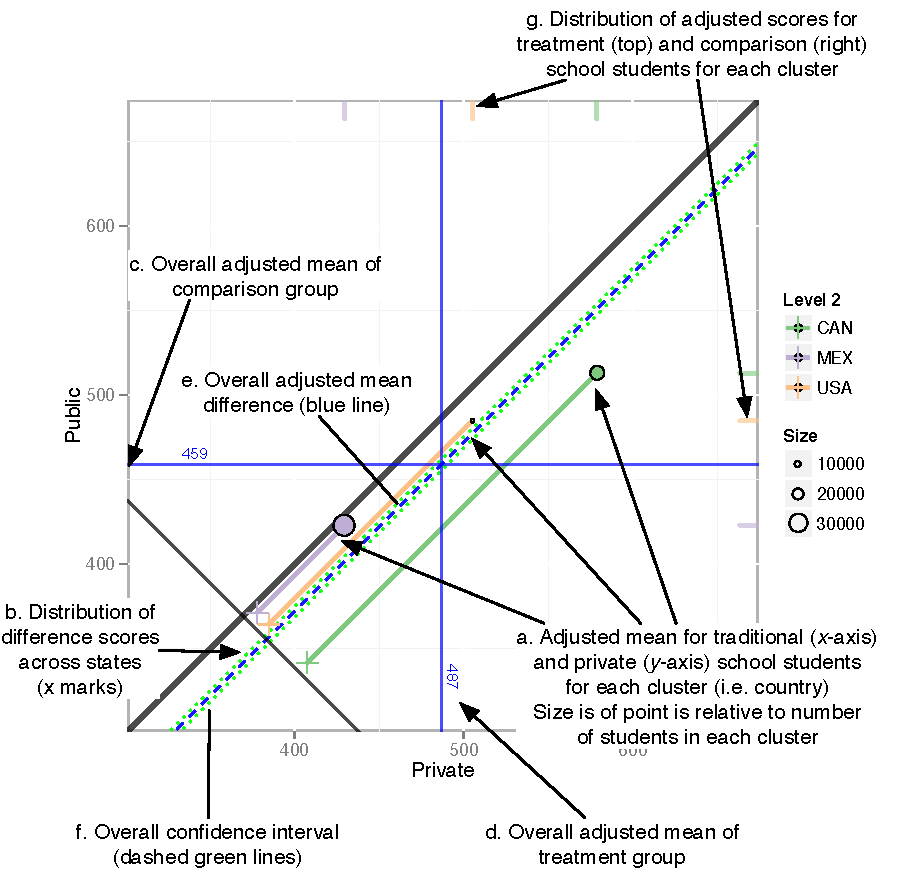
\includegraphics[width=\textwidth]{../Figures/AnnotatedCircPlot.pdf}
\caption{Multilevel PSA Assessment Plot}
\label{fig:g8math:circ}
\end{center}
\end{figure}

Figure 2 provides a more nuanced depiction of the differences both between and states. Similar to the multilevel PSA assessment plot, each blue dot corresponds to a state and is sized relative to the number of students within each state. The light gray dots correspond to each strata within each state. The graphic also provides confidence intervals for each state as well as the overall adjusted mean difference (the vertical blue line) and confidence interval (the vertical green lines).

\begin{figure}[t]
\begin{center}
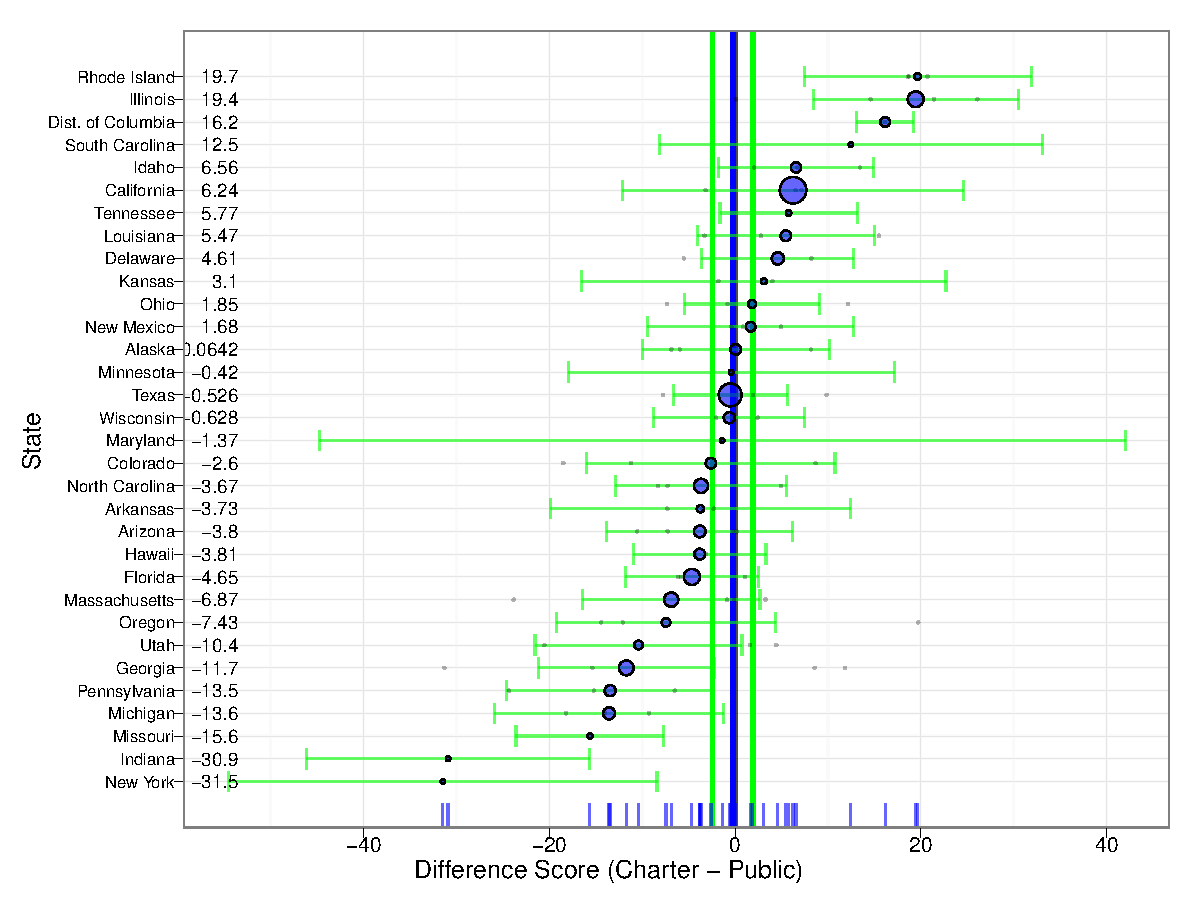
\includegraphics[height=4in]{../Figures/g8mathlrdiffplot.pdf}
\caption{Multilevel PSA Difference Plot: Grade 8 Math}
\label{fig:g8math:diff}
\end{center}
\end{figure}

\section{Results}

Figure \ref{fig:g8math:diff} provides a summary of all the results across the four dependent variables. This graphic displays the mean adjusted differences as blue dots with the confidence interval in green. Therefore, any instance where the confidence interval does not cross zero (as represented by the vertical black line) indicates there is a statistical significant difference. Examining Figure \ref{fig:overallresults}, we see there is general agreement across the nine different methods used. That is, given the various approaches to adjusting selection bias with the available student information provides consistent conclusions. Specifically, these results suggest there is no statistical difference between charter public school students in grade 4 math and reading. Grade 8 math provides mixed results whereby five of the nine methods have confidence intervals that do not span zero. For grade 8 reading however, there is a clear statistical difference as all nine methods result in confidence intervals that do not span zero (effect size < .20).

% latex table generated in R 2.12.2 by xtable 1.5-6 package
% Sun Jun 26 09:06:41 2011
\begin{table}[ht]
\begin{center}
\caption{Summary Propensity Score Analysis using Stratification}
\label{overallresults}
\begin{tabular}{lrrrrrrr}
  \hline
  & \multicolumn{ 2}{c}{Adjusted Mean} &  & \multicolumn{1x}{c}{} &  &  & \multicolumn{1}{c}{} \\ \cline{2-3} & Public & Charter & Diff & ATE & \textit{n} & \multicolumn{2}{c}{95\% CI} \\ \hline  & \multicolumn{7}{c}{Grade 4 Math} \\ \cline{2-8} \hline
Logistic Regression & 237.95 & 237.38 & -0.57 & -0.57 & 146656.00 & -1.72 & 0.57 \\ 
  Logistic Regression Step AIC & 237.96 & 237.35 & -0.60 & -0.60 & 146656.00 & -1.73 & 0.52 \\ 
  Conditional Inference Trees & 237.93 & 238.27 & 0.34 & 0.34 & 146638.00 & -0.96 & 1.64 \\ 
    & \multicolumn{7}{c}{Grade 4 Reading} \\ \cline{2-8}Logistic Regression & 218.27 & 218.96 & 0.70 & 0.70 & 141352.00 & -0.71 & 2.11 \\ 
  Logistic Regression Step AIC & 218.26 & 219.22 & 0.96 & 0.96 & 141352.00 & -0.44 & 2.37 \\ 
  Conditional Inference Trees & 218.26 & 219.01 & 0.75 & 0.75 & 141340.00 & -0.62 & 2.12 \\ 
    & \multicolumn{7}{c}{Grade 8 Math} \\ \cline{2-8}Logistic Regression & 278.77 & 279.10 & 0.33 & 0.33 & 97563.00 & -1.40 & 2.06 \\ 
  Logistic Regression Step AIC & 278.77 & 279.54 & 0.77 & 0.77 & 97563.00 & -0.91 & 2.46 \\ 
  Conditional Inference Trees & 278.72 & 280.89 & 2.17 & 2.17 & 97521.00 & 0.36 & 3.98 \\ 
    & \multicolumn{7}{c}{Grade 8 Reading} \\ \cline{2-8}Logistic Regression & 259.80 & 262.82 & 3.02 & 3.02 & 105486.00 & 1.55 & 4.49 \\ 
  Logistic Regression Step AIC & 259.80 & 262.67 & 2.87 & 2.87 & 105486.00 & 1.36 & 4.38 \\ 
  Conditional Inference Trees & 259.75 & 265.39 & 5.65 & 5.65 & 105468.00 & 4.36 & 6.93 \\ 
   \hline
\end{tabular}
\end{center}
\end{table}


\begin{figure}[t]
\begin{center}
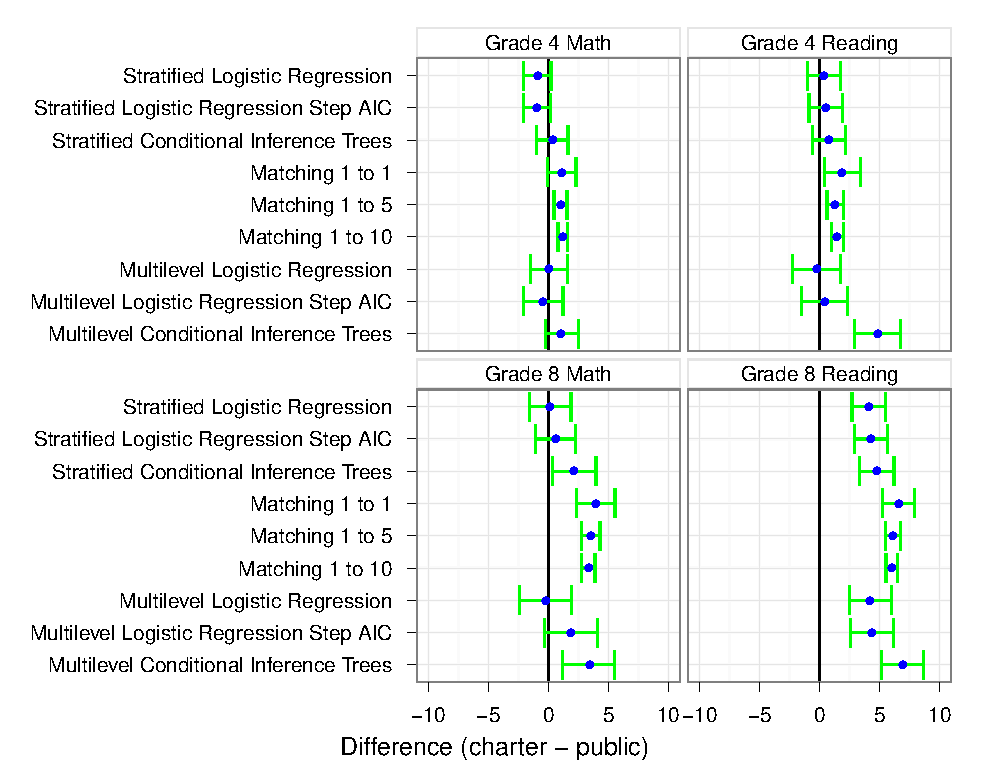
\includegraphics[height=4in]{../Figures/overallsummary.pdf}
\caption{Summary of Overall Results}
\label{fig:overallresults}
\end{center}
\end{figure}

%\clearpage
\printbibliography

\appendix
%\section{Multilevel PSA Assessment Plots}

\begin{figure}[t]
\begin{center}
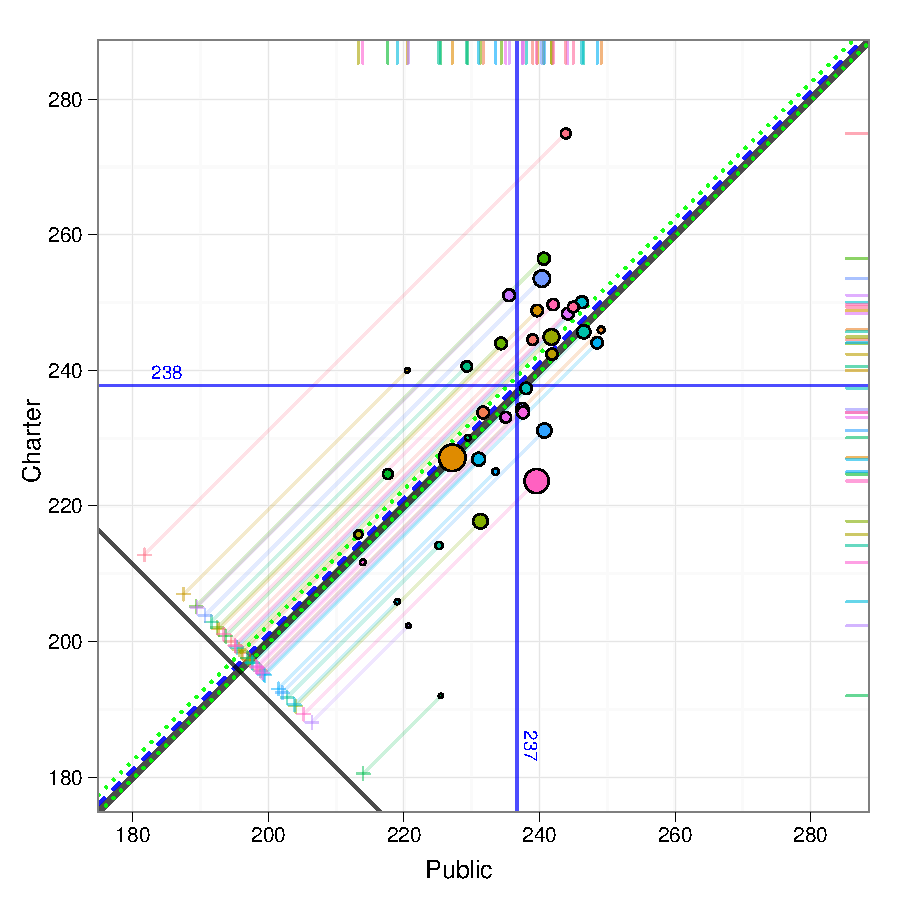
\includegraphics[width=\textwidth]{../Figures/g4mathtreecircplot.pdf}
\caption{Multilevel PSA Assessment Plot: Grade 4 Math}
\label{g4mathtreecircplot.pdf}
\end{center}
\end{figure}

\begin{figure}[t]
\begin{center}
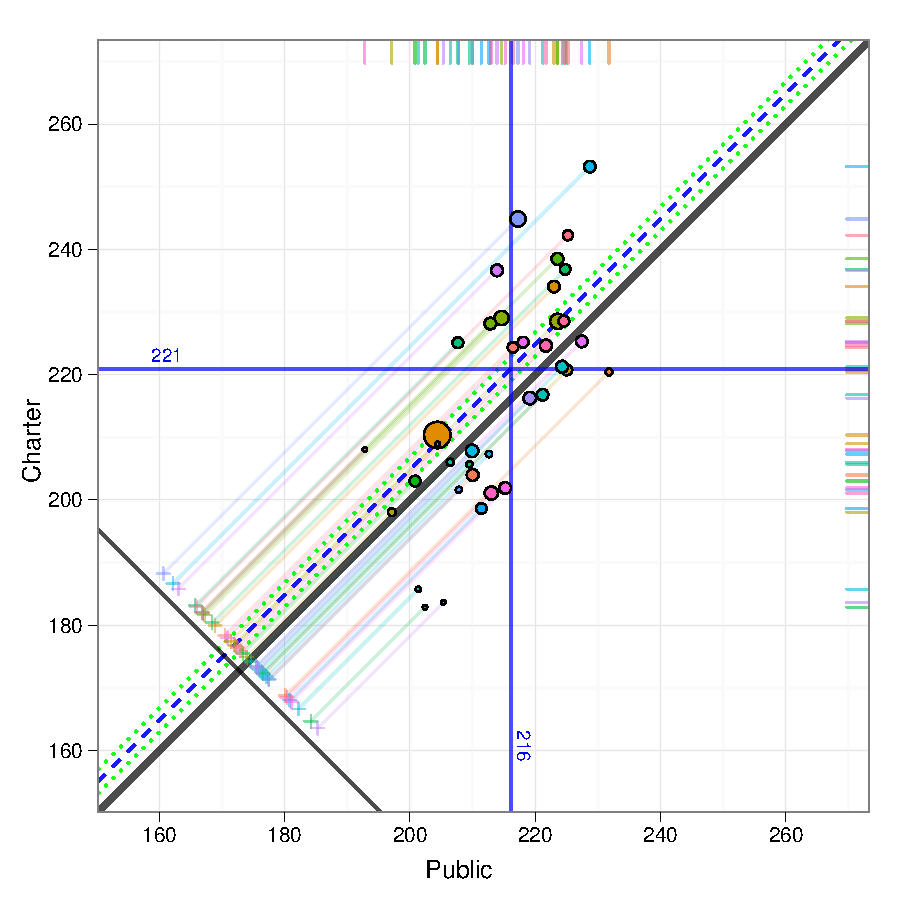
\includegraphics[width=\textwidth]{../Figures/g4readingtreecircplot.pdf}
\caption{Multilevel PSA Assessment Plot: Grade 4 Reading}
\label{g4readtreecircplot.pdf}
\end{center}
\end{figure}

\begin{figure}[t]
\begin{center}
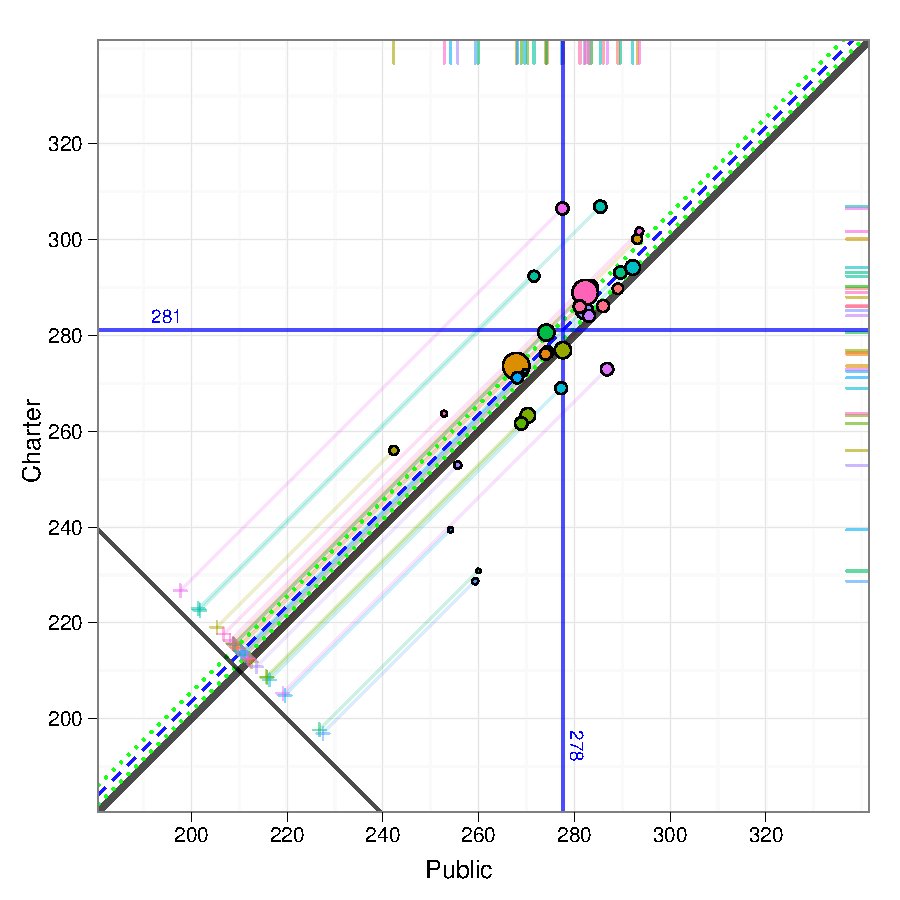
\includegraphics[width=\textwidth]{../Figures/g8mathtreecircplot.pdf}
\caption{Multilevel PSA Assessment Plot: Grade 8 Math}
\label{g8mathtreecircplot.pdf}
\end{center}
\end{figure}

\begin{figure}[t]
\begin{center}
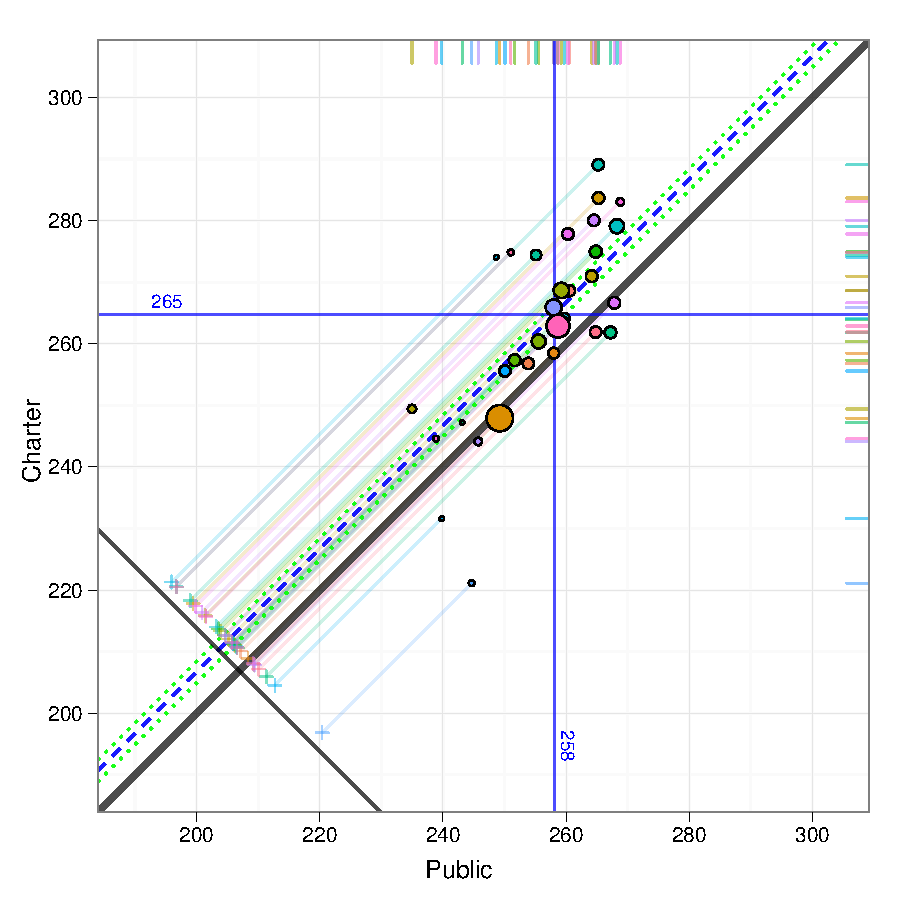
\includegraphics[width=\textwidth]{../Figures/g8readingtreecircplot.pdf}
\caption{Multilevel PSA Assessment Plot: Grade 8 Reading}
\label{g8readtreecircplot.pdf}
\end{center}
\end{figure}

\end{document}
